\section{Supplementary Protocol Detail}

\subsection{Fail-closed study lifecycle}

The external workflow progressed through sealed, started, and completed states.
Sealing bound the representation protocol, final training protocol, source tree,
environment, REVE checkpoint, HBN manifests, MIPDB acquisition and QC manifests,
subject lists, preprocessing, statistical specification, and all selected head
checkpoints. A started study could not be resealed. Infrastructure failures
could append diagnostic records and resume only against the same identities;
they could not replace an existing valid prediction.

The external evaluator had no optimizer, scheduler, checkpoint selection, or
aggregate metric capability. It first validated the lock and exact checkpoint
matrix, wrote the start marker, and then lazily extracted representations for
missing primary subjects. Completion required one immutable prediction for each
head--seed--subject triple. Confirmatory analysis refused incomplete or extra
entries.

\subsection{Interpretation of the joint criterion}

The five decision conditions answer complementary questions. The cohort-size
floor blocks a claim below the declared minimum but does not guarantee adequate
power or precision. Holm adjustment
controls the family-wise error rate across the three candidate comparisons.
The bootstrap lower bound requires the paired mean effect to remain positive
when both seeds and subjects vary. The win count guards against an average
driven by a minority of seeds, and the worst-seed threshold limits severe
optimization instability. The rule is intentionally stricter than selecting a
head by mean validation or external performance.

In this study, all candidates failed the bootstrap-lower-bound condition. The
multi-query candidate additionally exhibited losses on two seeds, although its
worst observed delta remained above the predeclared floor. Because the rule is
conjunctive, passing the adjusted test, win-count, and worst-seed checks cannot
compensate for an interval that includes zero.

\subsection{Evidence taxonomy}

The primary analysis compares frozen heads on MIPDB. The separate
NeuralBench-compatible training schedule aligns optimization mechanics, not the
overall benchmark task: official end-to-end NeuralBench training updates the
encoder, whereas the present encoder never receives a gradient. Historical HBN
screens motivated the choice of candidate families but are not used to estimate
the prospective effect. This distinction is necessary to avoid both benchmark
mislabeling and post-selection inference on repeatedly viewed outcomes.

\subsection{Evidence map and availability boundary}

The following map states which evidence supports which claim. It is included to
prevent a secondary benchmark result or a repeatedly inspected split from being
read as part of the sealed external estimand.

\paragraph{Primary prospective.} Frozen REVE heads on sealed MIPDB, comprising
40 runs and 3,000 subject-level predictions. This supports the confirmatory
statement about stable external gains under the declared protocol.

\paragraph{Secondary reproduction.} NeuralBench-compatible end-to-end runs with
a trainable encoder. These provide reproduction and implementation context, not
a frozen-probe or MIPDB score.

\paragraph{Retrospective secondary.} Previously inspected HBN R5 screens. These
provide motivation and implementation history, not untouched confirmation.

\paragraph{Exploratory layer-wise.} A separate four-layer, ten-seed analysis
compares matched linear probes at REVE layers $-4$, $-3$, and $-2$ with the
final-layer mean-linear baseline on the same previously evaluated
\LayerwiseSubjectCount{}-subject MIPDB cohort.
Its report and figures are aggregate-only and are bound to the completed
external prediction inventory; its intervals and sign-flip values are
descriptive and cannot modify the primary decision rule.

The compact release preserves protocol and artifact identities while excluding
raw recordings, model weights, participant identifiers, and subject-level
predictions. This boundary is deliberate: it permits source and analysis
audits without turning a restricted neuroimaging dataset into a public data
copy. An additional access-controlled demographic and recording-level
supplement is not included. The reported cohort flow should not be mistaken
for a comprehensive account of recruitment or acquisition differences.

\paragraph{Secondary ds006780 transfer.} The separate v5 transfer evaluates
the final-layer mean-linear and rich-statistics residual heads at HBN training
sizes 200 and 800 on 126 eligible ds006780 subjects and ten seeds. Its compact
aggregate bundle is retained under
\texttt{results/extensions/ds006780\_external\_v5/}; the bundle contains the
analysis report, failed precision-gate report, deterministic table, figure,
macros, and asset manifest, but no participant-level identifiers, target-bearing
manifest, predictions, checkpoints, or recordings. The primary n=800 interval
width was 0.1272 versus the predeclared maximum 0.06, so the extension is
reported as uncertainty-limited transfer evidence.

\section{Capacity-Data Regime Extension}

This secondary extension asks whether the observed behavior of expressive probe
heads changes with the amount of HBN training data. It reuses the frozen REVE
representation, preprocessing, external cohort, checkpoint rule, and training
contract of the primary study. The only planned factors are training size
($n\in\{200,400,800\}$), head family, and optimization seed. The matrix has
three heads, three training sizes, and ten seeds, for 90 frozen-head runs. The
external evaluation contains one prediction for every declared head-seed-subject
combination on the previously evaluated 75-subject primary cohort;
participant-level outputs are not included in this repository. The extension
does not add independent external subjects.

\subsection{Aggregate results}

The parameter counts are derived from the validated checkpoint metadata rather
than entered as manuscript constants. The aggregate external metrics and seed
variability are shown in Table~\ref{tab:capacity-absolute}. Paired candidate
contrasts against the training-size-matched mean-linear baseline are shown in
Table~\ref{tab:capacity-cells}. The six cell comparisons are positive for every
observed seed, but the uncertainty intervals are the primary indication of how
strongly those effects are supported.

\begin{table}[H]
  \centering
  \scriptsize
  \caption{Aggregate external Pearson performance in the capacity-data
  extension. Seed SD is computed across the ten matched optimization seeds.}
  \label{tab:capacity-absolute}
  \input{../results/extensions/capacity_data_regime_v3/capacity_data_regime_absolute.tex}
\end{table}

\begin{table}[H]
  \centering
  \scriptsize
  \caption{Paired candidate-baseline differences by training size. Intervals
  use the joint seed-subject bootstrap; Holm-adjusted p-values are exploratory
  and do not replace the primary sealed decision rule.}
  \label{tab:capacity-cells}
  \input{../results/extensions/capacity_data_regime_v3/capacity_data_regime_cells.tex}
\end{table}

The training-size contrasts quantify whether the candidate advantage itself
changes between nested training regimes. The endpoint and adjacent contrasts
are reported in Table~\ref{tab:capacity-contrasts}; none should be interpreted
as a universal scaling law. In particular, a larger training subset can change
both the baseline and candidate, so the relevant quantity is the paired change
in their difference, not the raw candidate score alone.

\begin{table}[H]
  \centering
  \scriptsize
  \caption{Exploratory changes in the paired candidate-baseline difference
  across training sizes.}
  \label{tab:capacity-contrasts}
  \input{../results/extensions/capacity_data_regime_v3/capacity_data_regime_contrasts.tex}
\end{table}

For context, the selected-head HBN validation scores and the corresponding
external scores are shown in Table~\ref{tab:capacity-transfer}. This is a
descriptive transfer view rather than a second selection criterion: the MIPDB
targets remain excluded from training and checkpoint selection.

\begin{table}[H]
  \centering
  \scriptsize
  \caption{Descriptive validation-to-external transfer for the candidate heads.}
  \label{tab:capacity-transfer}
  \input{../results/extensions/capacity_data_regime_v3/capacity_data_regime_validation_external_transfer.tex}
\end{table}

\subsection{Figures and robustness interpretation}

Figure~\ref{fig:capacity-absolute} displays the absolute external scores,
Figure~\ref{fig:capacity-delta} displays the paired deltas and bootstrap
intervals, and Figure~\ref{fig:capacity-seed-deltas} displays the per-seed
contrasts. The same 10,000-iteration hierarchical bootstrap is used throughout:
seeds and external subjects are resampled jointly while preserving candidate-
baseline pairing.

\begin{figure}[!ht]
  \centering
  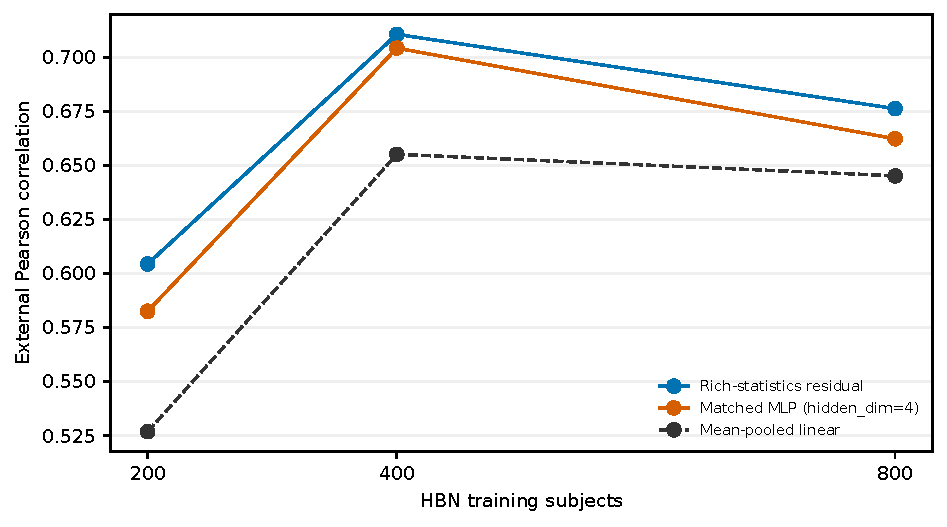
\includegraphics[width=0.94\linewidth]{../results/extensions/capacity_data_regime_v3/capacity_data_regime_absolute.pdf}
  \caption{Aggregate external Pearson scores across training sizes and probe
  heads.}
  \label{fig:capacity-absolute}
\end{figure}

\begin{figure}[!ht]
  \centering
  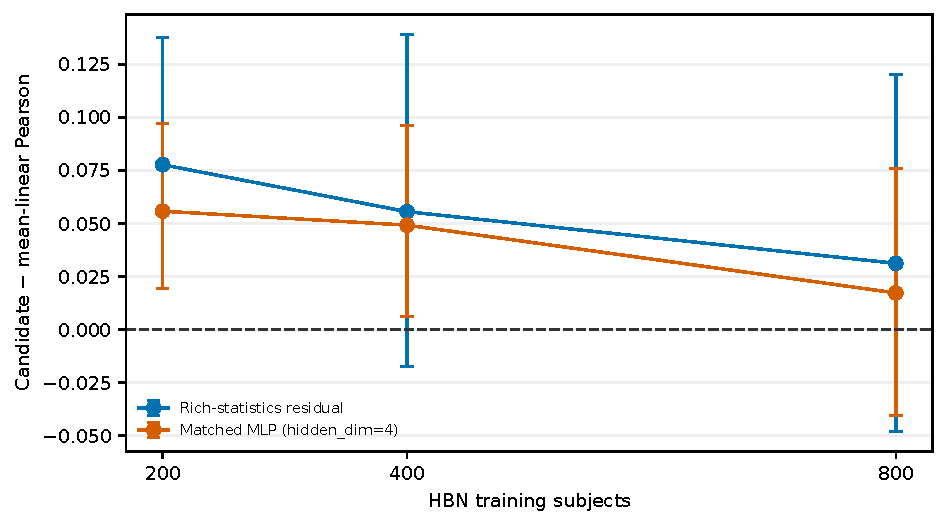
\includegraphics[width=0.94\linewidth]{../results/extensions/capacity_data_regime_v3/capacity_data_regime_delta.pdf}
  \caption{Paired external Pearson deltas relative to the matched mean-linear
  baseline, with joint bootstrap intervals.}
  \label{fig:capacity-delta}
\end{figure}

\begin{figure}[!ht]
  \centering
  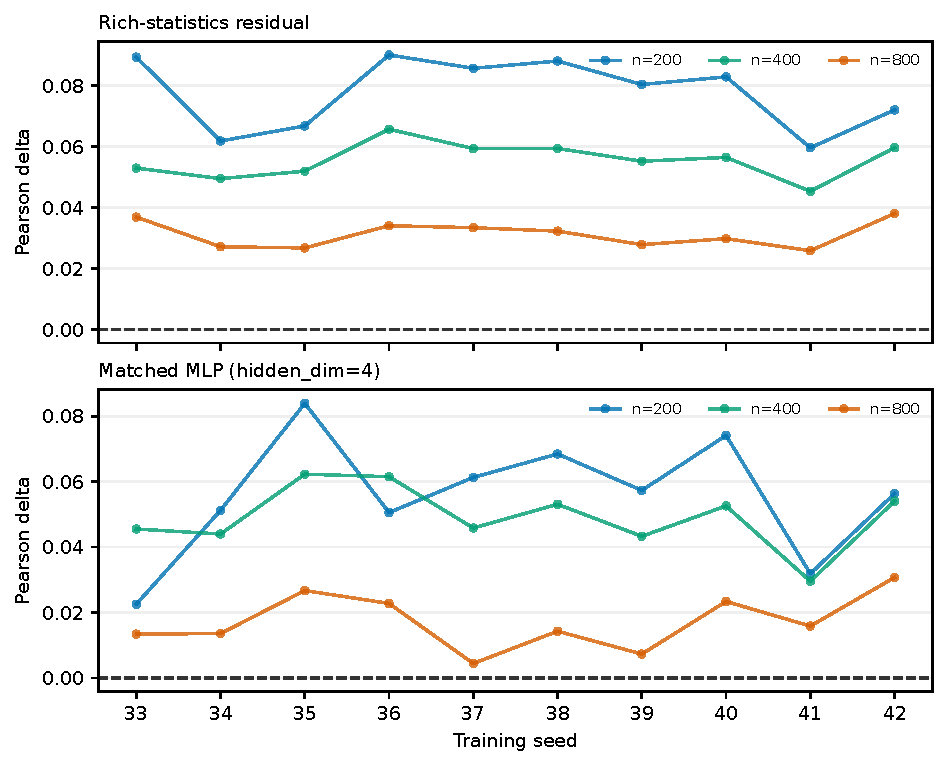
\includegraphics[width=0.94\linewidth]{../results/extensions/capacity_data_regime_v3/capacity_data_regime_seed_deltas.pdf}
  \caption{Seed-level paired external deltas for the two candidate heads.}
  \label{fig:capacity-seed-deltas}
\end{figure}

The exact seed sign-flip tests and Holm correction are exploratory descriptive
inference for this extension. Their configuration, family order, and canonical
digest are retained in the aggregate asset manifest. They do not alter the
primary predeclared superiority boundary: the sealed primary conclusion is
still determined by its hierarchical bootstrap, cohort, win-count, and
worst-seed criteria. The extension therefore supports a bounded statement
about head capacity under the tested data regimes, not a claim that a more
complex head is generally better or that additional training subjects have a
monotone effect.

